%\documentclass[12pt,ascmac]{jreport}
\documentclass[12pt]{jreport}
\usepackage{sty/eclepsf}
\usepackage{tascmac}
\usepackage{tabularx}
\usepackage[longnamesfirst]{natbib}
\usepackage[dvipdfm]{graphics}
\usepackage[dvipdfm]{graphicx}
\usepackage[dvipdfm]{color}
\usepackage{subfigure}
%\usepackage[dvipdfm, colorlinks, breaklinks,%
\usepackage[dvipdfm, breaklinks,%
bookmarks=true, bookmarksnumbered=true,%
bookmarkstype=toc, bookmarksopen=true,bookmarksopenlevel=3,%
pdftitle={Countermeasure based on risk analysis of collecting digital information },%
%%pdfsubject={},%
pdfauthor={Yuki Uehara},%
pdfkeywords={1.Network Tracking, 2.Digital Forensics, 3. Internet Security, 4.Network Monitoring}%
]{hyperref}

\AtBeginDvi{\special{pdf:tounicode EUC-UCS2}}

\usepackage{fancyhdr}

\usepackage{./sty/doxygenorig}

\usepackage{indentfirst}
\usepackage{url}
\usepackage{listings,sty/jlisting}

\lstset{%
 language={C++},
 %backgroundcolor={\color[gray]{.85}},%
 basicstyle={\small},%
 identifierstyle={\small},%
 commentstyle={\small\itshape},%
 keywordstyle={\small\bfseries},%
 ndkeywordstyle={\small},%
 stringstyle={\small\ttfamily},
 frame={tb},
 breaklines=true,
 columns=[l]{fullflexible},%
 numbers=left,%
 xrightmargin=0zw,%
 xleftmargin=1.5zw,%
 numberstyle={\scriptsize},%
 stepnumber=1,
 numbersep=1zw,%
 lineskip=-0.5ex%
}

\usepackage{amssymb}
%\usepackage{supertabular,multirow}

% A4  size: 297mm*210mm %1pt = 0.35mm
\setlength{\topmargin}{-3.4mm} % 10pt 25.4mm - 3.4mm = 22mm
\setlength{\oddsidemargin}{-0.4mm} % 25.4mm - 0.4mm = 25mm
\setlength{\evensidemargin}{-0.4mm} % 25.4mm - 0.4mm = 25mm
\setlength{\textheight}{231mm} % 660pt % original is 225.75mm 645pt
\setlength{\textwidth}{160mm} % 457pt

\renewcommand{\topfraction}{.99}
\renewcommand{\textfraction}{.0}
\renewcommand{\floatpagefraction}{.99}
\renewcommand{\bibname}{����ʸ��}

\pagestyle{fancy}  
%\rhead{\thepage}
%\rhead[]{\leftmark} 
\lhead[]{} 
%\lhead[\rightmark]{} 

\makeatletter
\def\chaptermark#1{\markboth {\ifnum \c@secnumdepth>\m@ne
\@chapapp\ \thechapter \@chappos\ \fi #1}{}}
\makeatother

\begin{document}


\pagenumbering{roman}

\begin{titlepage}

\begin{center}
\begin{Large}
´����ʸ ~~~~~ 2013ǯ�١�ʿ��25ǯ�١�
\end{Large}
\end{center}

\begin{center}
~ \bigskip ~ \\
\begin{LARGE}
\begin{tabular}{|c|}
\hline
�ޥ������֥�������Ѥ�����ֱ��Ծ�����˥����
\\ \hline
\end{tabular}
\end{LARGE}
\\

~ \bigskip ~ \\
~ \bigskip ~ \\
~ \bigskip ~ \\
~ \bigskip ~ \\


\end{center}
\begin{center}
\begin{Large}
\medskip
���������� �Ķ��������\\
\medskip
��̾��\underline{��ë ů��}\\
\medskip
\medskip
����\\
���������� �Ķ��������\\
¼�� ��\\
���� �ѹ�\\
���� ��Ƿ\\
��¼ ��\\
�⼮ �쵪\\
�Ŷ� �Ϲ�\\
Rodney D. Van Meter III\\
���� ����\\
���� ��\\
��߷ ��\\
���� ����\\
\medskip
{\today}

\medskip
\end{Large}
\end{center}


\end{titlepage}


\thispagestyle{empty}
´����ʸ�׻� - 2009ǯ�� (ʿ��21ǯ��)
~ \\
\begin{center}
\begin{Large}
\begin{tabular}{|c|} \hline
�ǥ������������ˤ��\\
�桼�����פȥꥹ��ʬ�Ϥ��к������
\\ \hline
\end{tabular}
\end{Large}
\end{center}
~  \\
%~ \bigskip ~ \\

%��ʬ�ι׸�����ˡ���¸��γ��פȷ�̡�
%����


%��ʸ���򤳤��Ȥ��Ƥ������ꡢ
���󵻽Ѥ�ȯŸ��ȼ�����ͥåȥ�����ȯ�������ǥ����������ưפ˵�
Ͽ�Ǥ���褦�ˤʤä�������ˤ�äơ����ޤ�ñ�ȤǤϥ桼���θĿ;���Ȥ�
��ʤ��ä������ʣ���Ȥ߹�碌�뤳�Ȥǡ��桼���ץ饤�Х�������������
ǽ�������롥��������˼���Ȥि��ˤϡ��桼�������Ū��ȯ�����Ƥ����
����Ȥ߹�碌���ݤˡ��ɤ����٤ޤǥ桼���ץ饤�Х������������Τ�����
�Τˤ��Ƶ�������ɬ�פ����롥�����ơ��桼���ץ饤�Х����뤿��ˡ�����
�ޤǸĿ;���ȸ����Ƥ��ʤ��ä���Τ�ޤ�ơ�����μ����ȼ�갷���˴�
���륬���ɥ饤������Τ˼����ʤ���Фʤ�ʤ���

����ʸ�Ǥϡ��桼����̵�ռ���ȯ�����Ƥ������μ����ˤ�äơ��桼���ץ�
���Х�������������ǽ�����󼨤��롥�Ŀ;���ˤʤꤦ��桼������ϡ���
������Ԥ��оݤˤʤ�桼���ȤΥͥåȥ���ξ�Ǥδط��ˤ�äƼ����Ǥ�
���ϰϤ��Ѥ�ꡤ�ꥹ�����Ѳ����롥�����ǡ�����Ū�˼�����ǽ�Ǥ���ȸ���
�ޤ������3����󤲡����줾��ξ���ˤ�äơ��桼���Υץ��ե�������
�������ˡ���󼨤���������ʸ�ǥץ��ե�������������Ѥ�������ϡ��ѥ���
�ȤΥإå����󡤥ۥ��Ȼ񸻶�ͭ�˴ؤ������Bluetooth�ǥХ�����õ������
�Ǥ��롥�����3�Ĥξ����¿���Υ桼�������Ū��ȯ�����Ƥ��뤿�ᡤ������
�ưפǤ��롥�����ξ���ˤ�äƤϡ��桼�������ꤹ�뤳�Ȥ��Ǥ���С��桼
���Υͥåȥ���ˤ������ư����䡤�ºݤ�������֤���ʤɡ��桼����
�饤�Х����������������������롥�����ơ��󼨤�����ˡ��¾ڤ��뤿��ˡ�
�ƾ������������Ϥ��륷���ƥ������������ڤ�����̡����Ҥ���3�Ĥξ������
�Ѥ��ƥ桼���Υץ��ե����뤬�����Ǥ��뤳�Ȥ��ǧ������

���������̤˴�Ť���3�Ĥξ�������Ѥ��ƥǡ�����������륱���������ꤷ��
�桼���Υץ饤�Х����Ф���ƶ���ͻ������������ơ��桼���Υץ饤�Х���
�ݸ�뤿��ˡ����ڷ�̤˴�Ť��������ɥ饤�����Ƥ�����


~ \\
�������:\\
\underline{1���ͥåȥ������}, \underline{2. �ե���󥸥å�},
\underline{3. �������ƥ�}, \underline{4���ͥåȥ���ƻ�},
\begin{flushright}
���������� ������������\\
~ \\
\begin{Large}
�帶 ͺ��
\end{Large}
\end{flushright}


\clearpage

\thispagestyle{empty}
Abstract of Bachelor's Thesis - Academic Year 2009
~ \\

%\begin{flushright}
%Academic Year 2008
%\end{flushright}

\begin{center}
\begin{Large}
\begin{tabular}{|c|} \hline
Risk Analysis and Countermeasures on User Tracking \\
by Digital Information Surveillance
\\
\hline
\end{tabular}
\end{Large}
\end{center}
~  \\
\indent As computer networks have covered various places and
population globally, users transmit various data in numerous occasions,
both intentionally and unintentionally.  As services that utilize the
network increased, the chance of data transmitted on the network being
accumulated and recorded has reached the significant level.  Those
individual data may not be considered as privacy information.
However, as those control data has increased, it became possible to
combine them and produce a single profile of a certain user.  When the
profiling become possible, the information that weren't considered as
a privacy information then becomes a privacy information.

To ensure that the users' privacy aren't intruded, it is necessary to
determine which information could lead the profiling of the user, and
construct a guideline based on the study.  This thesis clarifies the
types of information that could be accumulated to profile a user, and
how those information could be captured on the computer network.The
method proposed in the thesis classifies collectors into three
categories, and different methods of profiling is stated based on the
characteristics of those categories.  The information used for
capturing a user's profile includes: packet header information,
information used for sharing hosts' computing resources, and device
discovery information for Bluetooth devices.  The threats that could
outcome from the profiling include: revealing users' activity history,
discovering when the users are actively using the network, and
determining actual location of the physical computer that is being a
source of the information.The system for capturing and analyzing those information was developed
to present that they could be a threat against privacy information.  The
result showed that both specifying an individual user and profiling the
user's activities is possible based on the method presented in the
thesis.

Based on the evaluation,we discussed cases of collecting these imformation and impact of users privacy.
Additionally, the guidelines for handling those information is
proposed, to ensure that the users' privacy are protected and secured.


~ \\
Keywords : \\
\underline{1. Network Tracking}, \underline{2.Digital Forensics}, \underline{3.Internet Security}, \underline{4.Network Monitoring}

\begin{flushright}
Keio University, Faculty of Policy Management\\
~ \\
\begin{Large}
Yuki Uehara
\end{Large}
\end{flushright}

\clearpage

\tableofcontents\thispagestyle{empty} %�ܼ�
\clearpage
\listoffigures\thispagestyle{empty} %���ܼ�
\clearpage
\listoftables\thispagestyle{empty} %ɽ�ܼ�
\clearpage
\pagenumbering{arabic}
\chapter{����}
\label{introduction}
�ܾϤǤϡ��طʤǤ���桼�����ռ�������ȯ�����Ƥ�����󤬡��桼���ץ饤
�Х��򶼤�����ǽ�������뤳�Ȥ�Ҥ٤롥�����ơ��������ǥ������̿������
�ץ饤�Х��Τ���������Ƥ���Ȥ�����Ū�����餫�ˤ���ȤȤ�ˡ�����ʸ��
�����򵭤���
\section{�桼����ȯ���������Ȥ�������}
\label{introduction:intro}
%����������
��ǯ�����󵻽Ѥ�ȯŸ�ˤ�äƥ桼���˴ؤ����͡��ʾ��󤬡��ǥ������̿���
�����������졤��Ͽ�Ȥ��ƻĤ���褦�ˤʤä�������ˤ�äơ��桼���˴ؤ�
��������������Ϥ��뤳�Ȥǡ����������ͤ����߽Ф����Ȥ��Ǥ��롥���Τ�
�ᡤ���桼�����׵�˱����������ӥ����󶡤���ǽ�Ȥʤä�����ɽŪ�ʤ��
�Ȥ��Ƥϥ桼���ι��������¾�桼���ι����������Ӥ���쥳���ǡ�����
�󵻽Ѥ����Ѥ��Ƥ���Amazon\cite{amazon:2009}�䡤���ߤΰ��־���ȹ����
�Ȥ߹�碌�뤳�Ȥˤ�äơ��桼���μ��Ϥ�������������륵����
��NAVITIME\cite{navitime}�ʤɤ��󤲤��롥�����������Τ褦�ʾ��󵻽Ѥ�
ȯŸ�ˤ�äơ�����ޤǤϸĿ;���ȸ��ʤ���ʤ��ä����󤬡��桼���Υץ饤
�Х��򶼤����Ȥ�����ǰ�����롥

%�ץ饤�Х��ˤĤ���
�Ŀ;�������Ѥ��륤�󥿡��ͥåȥ����ӥ��䥳��ƥ�Ĥ����ä���ˤ����ꡤ
�桼���Υץ饤�Х����ݸ��ɬ���������롥���Τ��ᡤ������ͭ�Ԥϸ�̩��
������������褦�ˤʤä����Ŀ;���򰷤�¦�ϡ��Ŀ;���˴ؤ��뵬��
�򵭺ܤ����Ʊ�������ѥץ饤�Х����ݸ���͡��ʵ��Ѥ���Ƥ��Ƥ��롥��
��ʸ�ǽҤ٤�Ŀ;���Ȥϡ��Ŀ;����ݸ�ˡ���������������Ƥ��롤"��
¸����Ŀͤ˴ؤ������Ǥ��äơ���������˴ޤޤ���̾����ǯ��������¾
�ε������ˤ������θĿͤ��̤��뤳�Ȥ��Ǥ����Ρ�¾�ξ�����ưפ˾�
�礹�뤳�Ȥ��Ǥ�������ˤ������θĿͤ��̤��뤳�Ȥ��Ǥ��뤳�ȤȤʤ�
��Τ�ޤ��"\cite{privacy_policy:2009}��ؤ��������ơ��ץ饤�Х���
��Privacy and Freedom\cite{privacy:1967}�ǽҤ٤Ƥ��롤"�軰�Ԥ��������
�ؤ���Ŀ;����ɤ����ټ������뤤�϶�ͭ���뤳�Ȥ��Ǥ��뤫����������
���븢��"��������롥

�桼���Υץ饤�Х�����ǰ�������������󤲤롥�ǥ�����ǥХ��������ä�
��äơ��桼���ϰտޤ�����¿���ξ����ȯ�����Ƥ����礬���롥���κݤˡ�
���Ȥ˴ؤ����󤬴ޤޤ�Ƥ�����䡤���οͤȴؤ�꤬��������ȯ����
�Ƥ����礬���롥�ޤ����ͥåȥ����Ǥξ����ʣ�����Ȥ߹�碌�뤳��
�ǡ�������Τ˸ĿͤΥץ��ե������������뤳�Ȥ��Ǥ��롥����ˤ�äơ�
ʣ���ξ�����Ȥ߹�碌�뤳�Ȥˤ�äƥͥåȥ���ˤ�����桼����Ĵ���䡤
Ĵ���ˤ�ä�����줿���׾����������뤳�Ȥˤ�뿷���������ӥ��䡤�Ⱥ�
�ܺ��ʤɤ����ѤǤ���ȿ�̡��桼���Υץ饤�Х�����������ĤĤ��롥

%�ץ饤�Х��ˤĤ��Ƥ�������
���ߡ��桼���Υץ饤�Х����ݸ��¿���ε��Ѥ���Ƥ���Ƥ��뤬���ǥ���
��ǥХ��������äˤ�äơ��桼�������Ȥξ�����Τ餺�˸������Ƥ�����
�䡤���ޤǤϸĿ;���Ȥʤ�ʤ��ä���������礹�뤳�Ȥˤ�äơ��桼��
���ȤΥץ饤�Х�������������ǽ�������롥����ϡ��ɤΤ褦�ʾ��󤬼��Ȥ�
�ץ饤�Х��򶼤�����Ƥ��뤫�Τɤ����٤θ��¤���ĥ桼���ޤ��Τ뤳�Ȥ�
�Ǥ��뤫�Ȥ�������ʬ����ۣ�������Ǥ��롥����������褹��ˤϡ�
�ɤΤ褦�ʾ���ˤ�äƥ桼���Υץ饤�Х������������Τ����Τˤ��ơ��桼
�����Ȥ⤽����Τ�ɬ�פ����롥

%�Ǥ⥳��ƥ�ĶȼԤϻȤ�������͡�
����������ƥ�Ĥ䥵���ӥ��󶡼ԤϸĿ;�������ΨŪ�˼�������ɬ�פ�����ȿ�̡�
Ʊ���˥桼���Υץ饤�Х����ݸ���θ������ʤ���Фʤ�ʤ�������
���뤳�Ȥ��Ǥ�����󤹤٤Ƥ����Ѥ�����硤�桼���Υץ饤�Х��ζ��ҤˤĤʤ�
���ǽ�������롥���Τ��ᡤ����ƥ�ġ������ӥ��󶡼Ԥϼ�������桼����
������������뤫���⤷�������¤򤷤���Ǿ�����������ɬ�פ����롥


%�����ǽ��֤Ǥ���
\section{�ܸ������Ū}
\label{introduction:purpose}
����ʸ����Ū�ϡ��ǥ�����������ˤ����뿷�����ץ饤�Х��Τ���������
���뤳�ȤǤ��롥�ɤΤ褦�ʾ��󤬥桼���Υץ饤�Х��򿯳����뤫�����Τ�
�����ȤȤ�ˡ�����μ�갷���ˤĤ��Ƹ�Ƥ���롥¿���Υǥ����뵡�������
Ū�����Ѥ���褦�ˤʤä����Ȥǡ��桼���⥵���ӥ��󶡼Ԥ�ɤΤ褦�ʾ���
��ȯ������Ƥ��ꡤ�ɤΤ褦�ʱƶ���⤿�餹���İ�������Ƥ��ʤ��������ǡ�
����ʸ��ä�����줿�θ����󼨤��뤳�Ȥˤ�äơ�ISP��Ϥ���Ȥ���ͥå�
��������Ԥ䡤�����ӥ��󶡼ԡ����ץꥱ�������ȯ�Ԥϡ��ɤΤ褦�ʾ�
�󤬥桼���Υץ饤�Х��򶼤��������İ������Ŀ;�������ΤʻؿˤΤ�Ȥ�
�ݸ�뤳�Ȥ��Ǥ��롥�ޤ����桼�����Ȥ⡤�ɤ�ʾ������ʤ���Фʤ�
�ʤ������Τ뤳�Ȥǡ����ȤΥץ饤�Х�����ʤ���Фʤ�ʤ����ץ饤�Х�
���ݸ�ȡ��������ϥȥ졼�ɥ��դǤ��ꡤ�ɤ��ޤǵ��Ƥ����Τ����Τʶ�ʬ
����ɬ�פǤ��롥�桼���Υץ饤�Х����ưפ˿�������ʤ��Ҳ��¸����뤿��
�ˤϡ��ͥåȥ�������ԡ������ӥ��󶡼Ԥȥ桼��¦����������Ŀ;����
�ؤ����ݸ�򤷤ʤ���Фʤ�ʤ����äˡ��桼�������Ȥ˴ؤ������������
�뤳�Ȥ����桼���Υץ饤�Х����Ф��붼�Ҥ��㸺�Ǥ����ǽ�����⤤���桼
�������Ѥ�������������뤳�Ȥˤ�äơ�����μ�����򤬤Ǥ��뤫��Ǥ�
�롥������������ϥ桼�����ɤξ����ȯ�����Ƥ褤���ΤäƤ��뤳�Ȥ�����
�Ǥ��롥

����ʸ�Ǥϥ桼����̵�ռ���ȯ�����Ƥ������ˤ�äơ��桼���Υ�
�饤�Х����ɤ����ٶ�������Ƥ��뤫��Ĵ�����¾ڤ��롥���μ���Ȥߤˤ��
�ơ��桼�����Ȥ��ɤΤ褦�ʾ����¾�Υ桼���˼��������ȥץ饤�Х���
��������ǽ�������뤫��ޤȤ��ȤȤ�ˡ��ɤξ��󤬤ɤ�Ω��Υ桼����
���Τ뤳�Ȥ��Ǥ��뤫�Ȥ�����ʬ�������Τˤ��롥�㤨�С��桼���ι�ư����
�ϥͥåȥ�������Ԥ����Ǥʤ�Ʊ���ͥåȥ������³���Ƥ���桼���ޤ�
�Τ����뤫�Ȥ���Ĵ���ʤɤ��󤲤��롥


%�����ơ����󥿡��ͥåȤ�ޤ�ǥ������̿��ˤ�����桼���Υץ饤�Х��θ���
%�򼨤���Ʊ���ˡ��ǥ�����������������ǡ��桼���Υץ饤�Х��򶼤���
%�������������Ѥ����ˡ���󼨤������ڤ��롥

����ʸ�Ǥ�����Ū�˥桼����ȯ�������������Ѥ��뤳�Ȥǡ��ץ饤�Х�����
��������ǽ���Τ����ˡ��3�ļ��������Ф��Ƹ��ڡ��ͻ����롥����ˤ�äơ�
�ɤ��ޤǸĿ;����������뤳�Ȥ��Ǥ���Τ������Τ��롥�ܸ���ϥѥ��å�
�Υإå����󡤶�ͭ�ۥ���̾��Bluetooth�ǥХ���̾���Ѥ������ˡ��Ŀ;���
����������ˡ���󼨤������ڤ��롥�����ξ���ϡ��桼��������ȯ���Ƥ�
�����Ǥ��뤿�ᡤ�ưפ˼�����ǽ�Ǥ��롥���Τ��ᡤ�����ξ��󤬥桼��
�Υץ饤�Х��򶼤����Ƥ��뤫�Τ����ɬ�פ����롥

�����θ��ڷ�̤�Ƨ�ޤ��ơ��Ŀ;������ѻ��ˤ�����ץ饤�Х����ݸ����
Ū�Ȥ��������ɥ饤�����Ƥ��롥����ˤ�ꡤ�桼�����Ȥ�ͥåȥ����
���ԡ����ץꥱ�������ȯ�Ԥʤɤ�Ω���̤ˡ��ץ饤�Х���뤿��ˤϡ���
�ξ�����ꡤ�ޤ���ȯ�����Ƥ����꤬�ʤ����Ȥ��������������Τˤ��뤳��
����Ū�Ȥ��롥

\section{����ʸ�ι���}
\label{introduction:organization}
\indent ����ʸ����\ref{conclusion}�Ϥ��鹽������롥
��\ref{background}�ϤǤϡ��ǥ��������μ�����ˡ�ȥ桼���Υץ饤�Х���
���ҤȤʤ����ˤĤ��ƽҤ٤롥��\ref{related_works}�ϤǤϡ�
��\ref{background}�ϤǽҤ٤�����˼���Ȥ��Ϣ�����Ҳ𤹤롥
��\ref{assumption}�ϤǤϡ��ɤΤ褦�ʾ�����Ȥ߹�碌��ȥ桼���ζ��Ҥ�
�ʤ뤫��Ĵ���������μ�ˡ����Ƥ��롥��\ref{evaluation}�ϤǤϡ�
��\ref{assumption}�ϤǽҤ٤���ˡ��Ƥ�������μ¸���̤ˤĤ��ƽҤ٤��
�Ȥ�ˡ��ͻ���Ԥ�����\ref{consideration}�ϤǤϡ���\ref{evaluation}�Ϥ�
���ڤ�����ˡ���к��Ȥ��ơ������ɥ饤�����Ƥ��롥�Ǹ��
��\ref{conclusion}�Ϥ�����ʸ�η����ȡ������Ÿ˾��Ҥ٤롥


%%% Local Variables:
%%% mode: japanese-latex
%%% TeX-master: "../nakajima_bthesis"
%%% End:

\chapter{�ط�}
\label{background}
�ܾϤǤϡ��ż֤��ٱ�˴ؤ���͡��ؤαƶ���Ŵƻ��Ҥ��ԤäƤ�������ξ���ȯ����
�Ĥ��ƽҤ١��������������������򼨤������β��Τ��������ʸ����Ƥ���ӥå��ǡ���
���Ϥ˴�Ϣ�������Ѥ並��ˤĤ��ƽҤ٤롥

\section{�ż�}
�ż֤�¿���οͤ��̶С��̳ؤμ��ʤȤ��Ƴ��Ѥ���Ƥ��롥���������ٱ�䱿�Ը�
��碌�ʤ��������⤢�롥����Ǥϡ��ż֤���������Ŵƻ��Ҥ��ԤäƤ��������
�б��ˤĤ��Ƽ�����

\subsection{�ż֤�������}
\label{background:railroads:problems}
\begin{figure}
    \begin{center}
      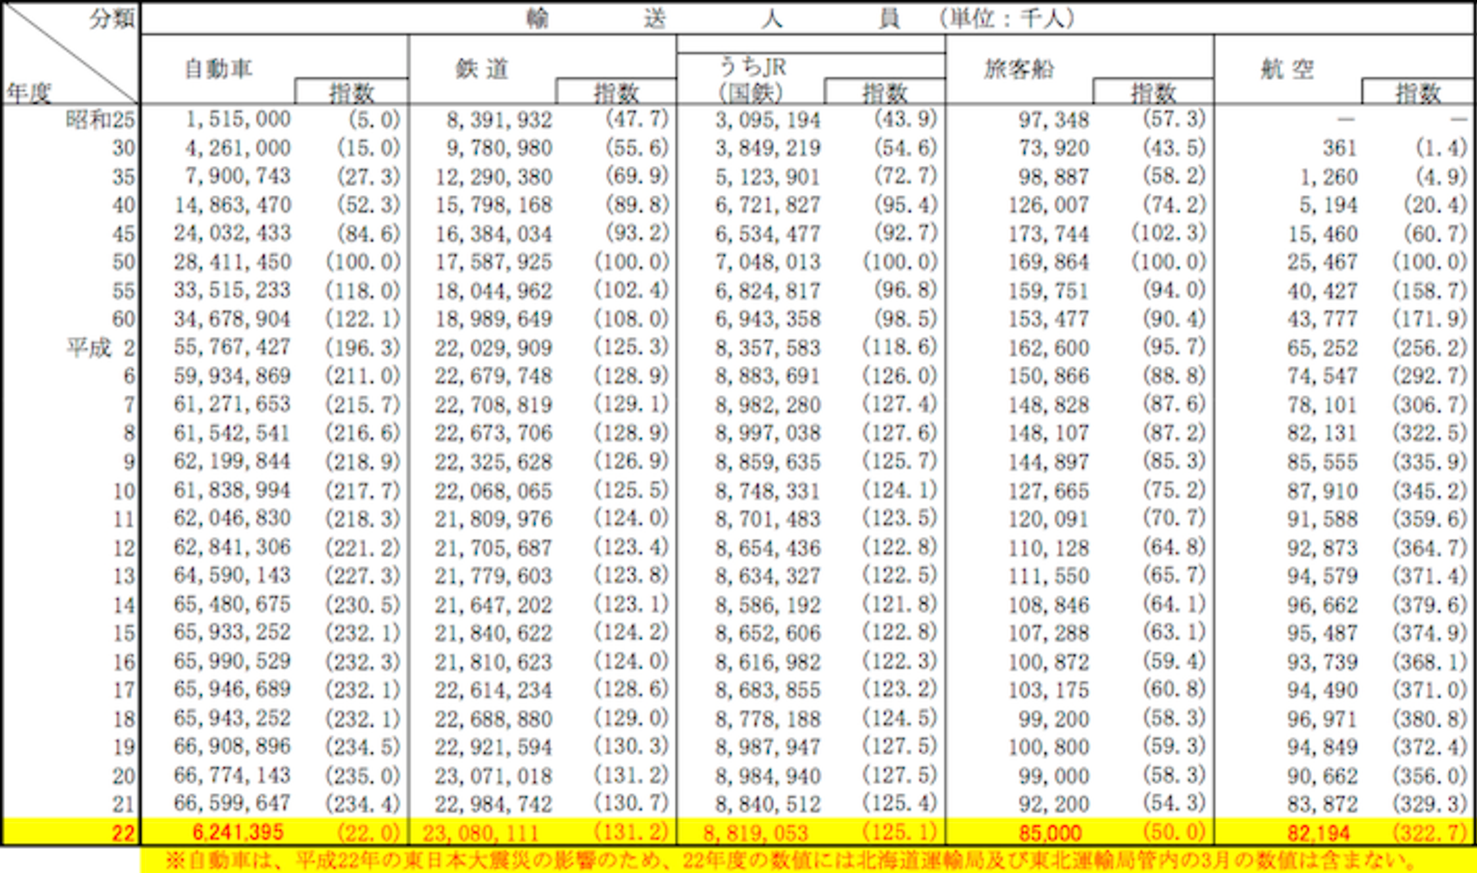
\includegraphics[scale=0.60]{./pdf/kokudokotsusho_users_num}
      \vspace{-5mm}
      \caption{���ܤ�͢��������͢���Ͱ���}
      \label{fig:kokudokotsusho_users_num}
    \end{center}
\end{figure}

���ܤˤ����ơ�¿���οͤ��̶С��̳ؤμ��ʤȤ����ż֤���Ѥ��Ƥ��롥�ż֤�
������û���֤�Ĺ��Υ��ư���뤳�Ȥ��Ǥ���Ȥ������Ǥ��롥�ޤ��֤Ȱ㤤ƻϩ
�ν��ڤ�ʤ�������ɽ�̤�˱��Ԥ��Ԥ��뤿�����ѼԤ����Τʰ�ư���֤��θ
����������Ѥ��뤳�Ȥ��Ǥ��롥���Τ��ᡤ�͡��ʾ��̤��͡��ʿͤ˳��Ѥ����
���롥���ڸ��̾ʤ���ɽ���Ƥ���ι�Ҥ�͢��������͢���̤�
��\ref{fig:kokudokotsusho_users_num}\cite{kokudokotsusho:num_of_users}
�ˤ��ȡ�ǯ����230���ͤ����ܿͤ����̤μ��ʤȤ����ż֤���Ѥ��Ƥ��롥�ż�
�����ѿͿ���¾��͢�����ؤ���¿�������ܤˤ������ż֤ϤȤƤ���פ�����
�̤����Ƥ��롥
\\

���������������⤢�롥���֤����ΤǤ���Ȥ������Ȥ���¿���οͤ˳��Ѥ����
�����ż֤��������Τ����������ʤɤˤ�ä��ٱ�䱿�Ը���碌�ʤɤ������Ƥ�
�ޤ����Ȥ�¿�����롥���ηкѥ���饤��ε���\cite{delay:higaigaku}�����
�������ֶ����ˤ��ȡ��ż֤��ٱ�ˤ���Զ���ؤ��̶Фˤ�����Ҳ�Ū���Ѥ�
ǯ��2180���ߤˤ�ʤ�ȿ�¬����Ƥ��롥���Τʿ����Ȥϸ����ʤ������ż֤���
�ѼԤˤȤä��ż֤��ٱ䤬�ȤƤ�¿����»����Ϳ���Ƥ���ȸ����롥
\\
%http://toyokeizai.net/articles/-/10756

\subsection{Ŵƻ��Ҥ��ٱ���Ф����б�}
\label{background:railroads:correspondence}
\begin{figure}
    \begin{center}
      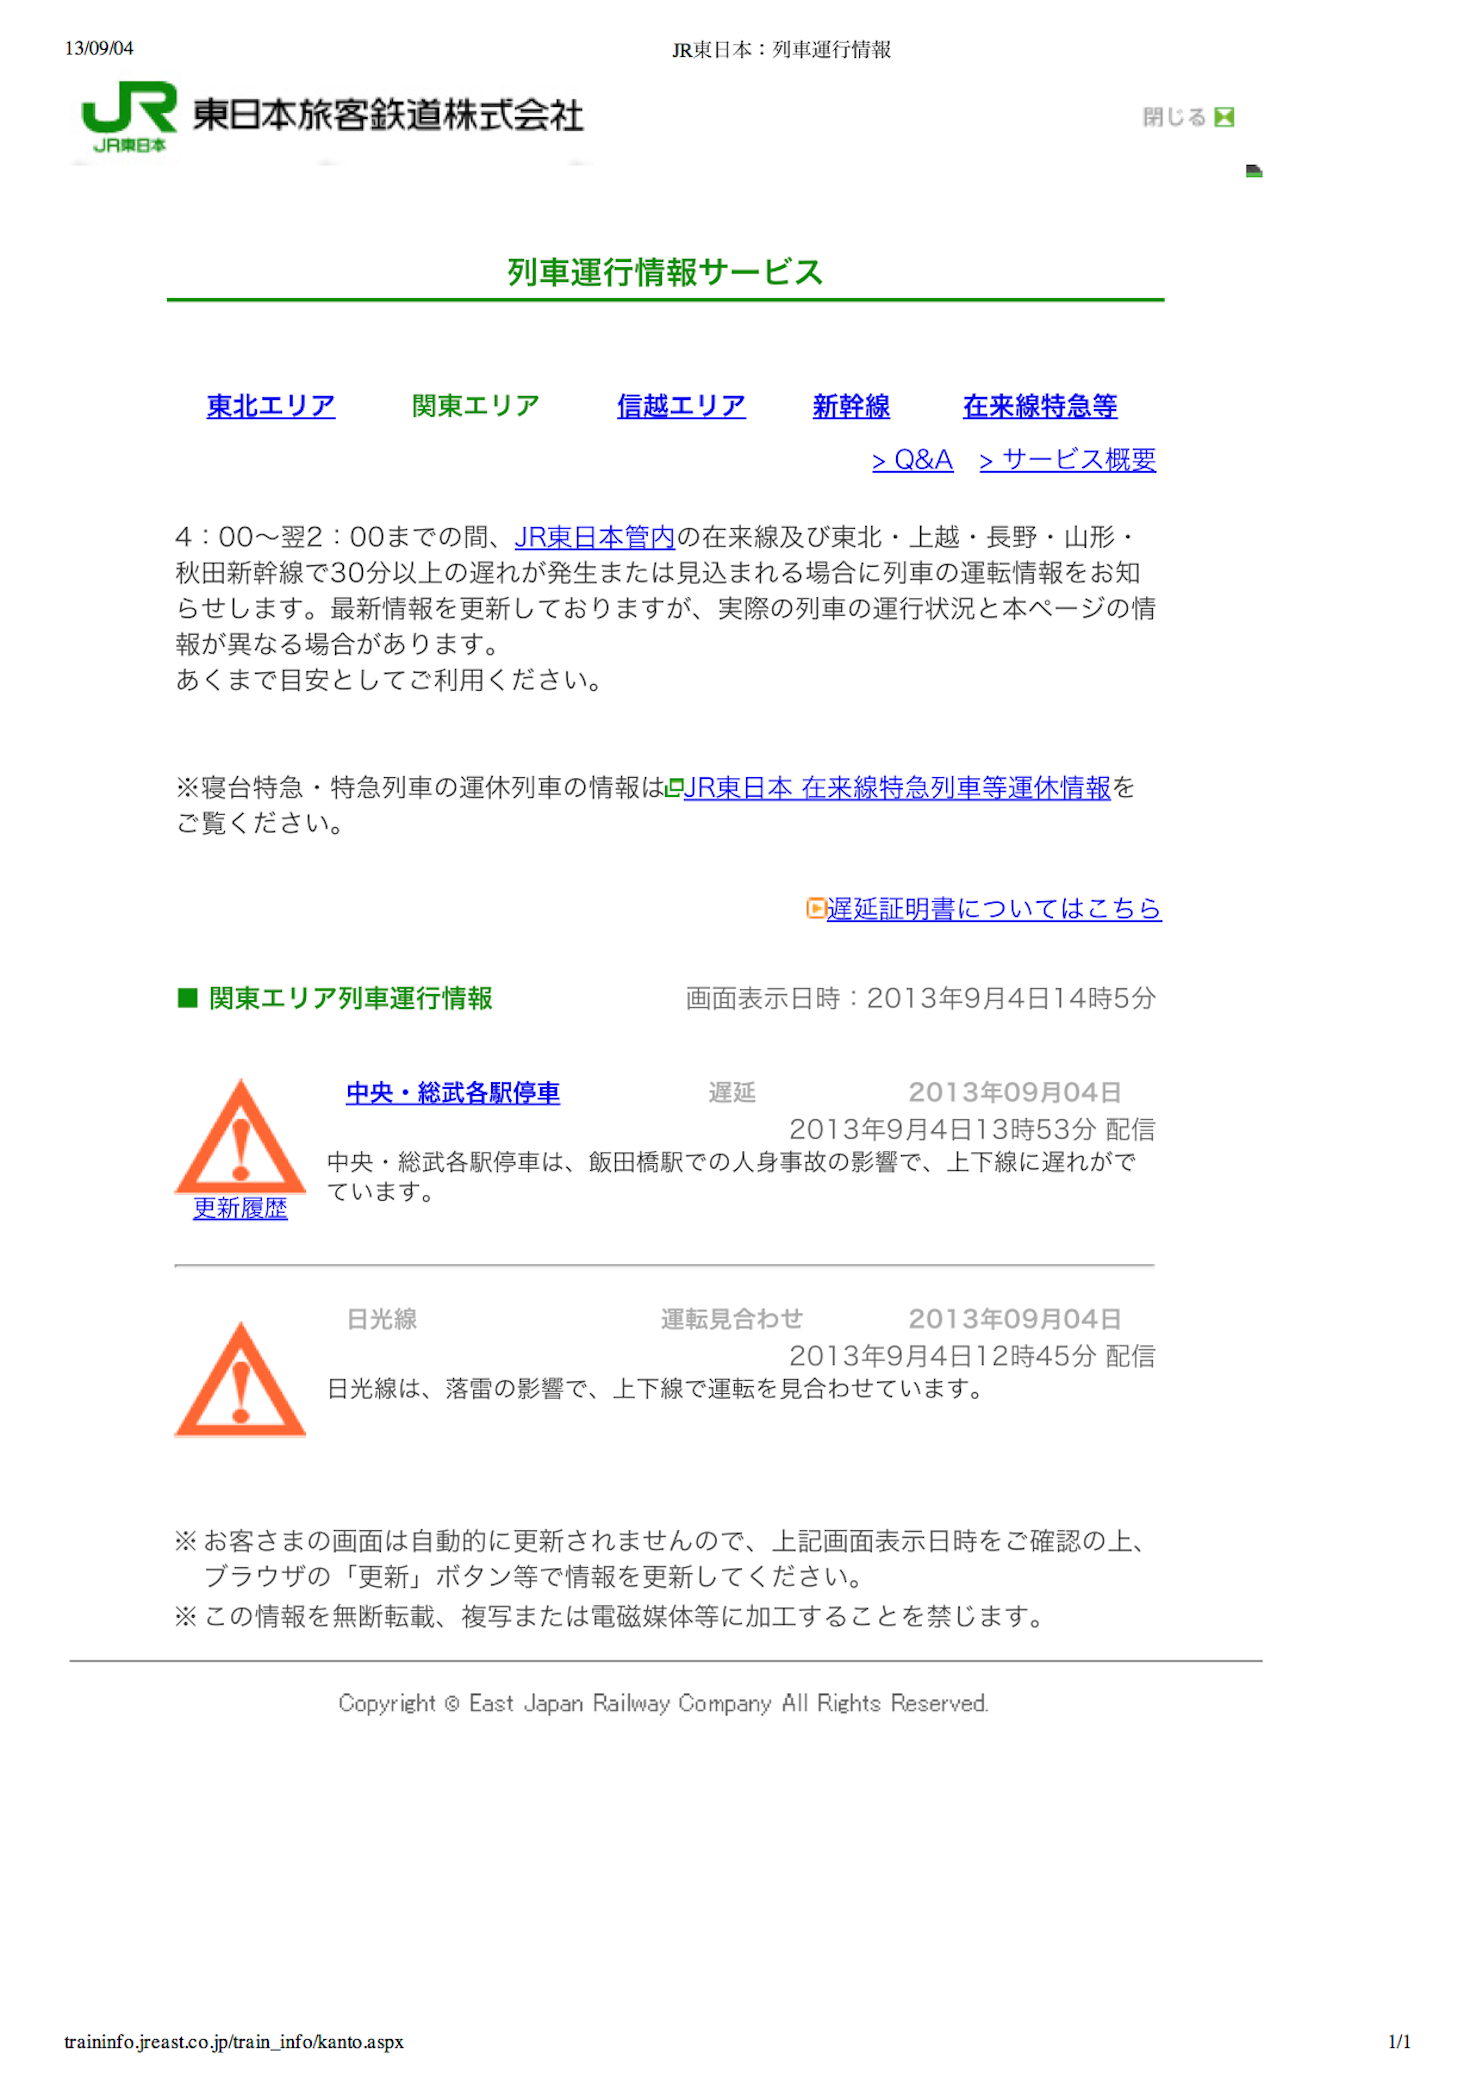
\includegraphics[scale=0.60]{./pdf/jr_delays_page}
      \vspace{-5mm}
      \caption{JR��ֱ��Ծ��󥵡��ӥ��ڡ���}
      \label{fig:jr_delays_page}
    \end{center}
\end{figure}
\begin{figure}
    \begin{center}
      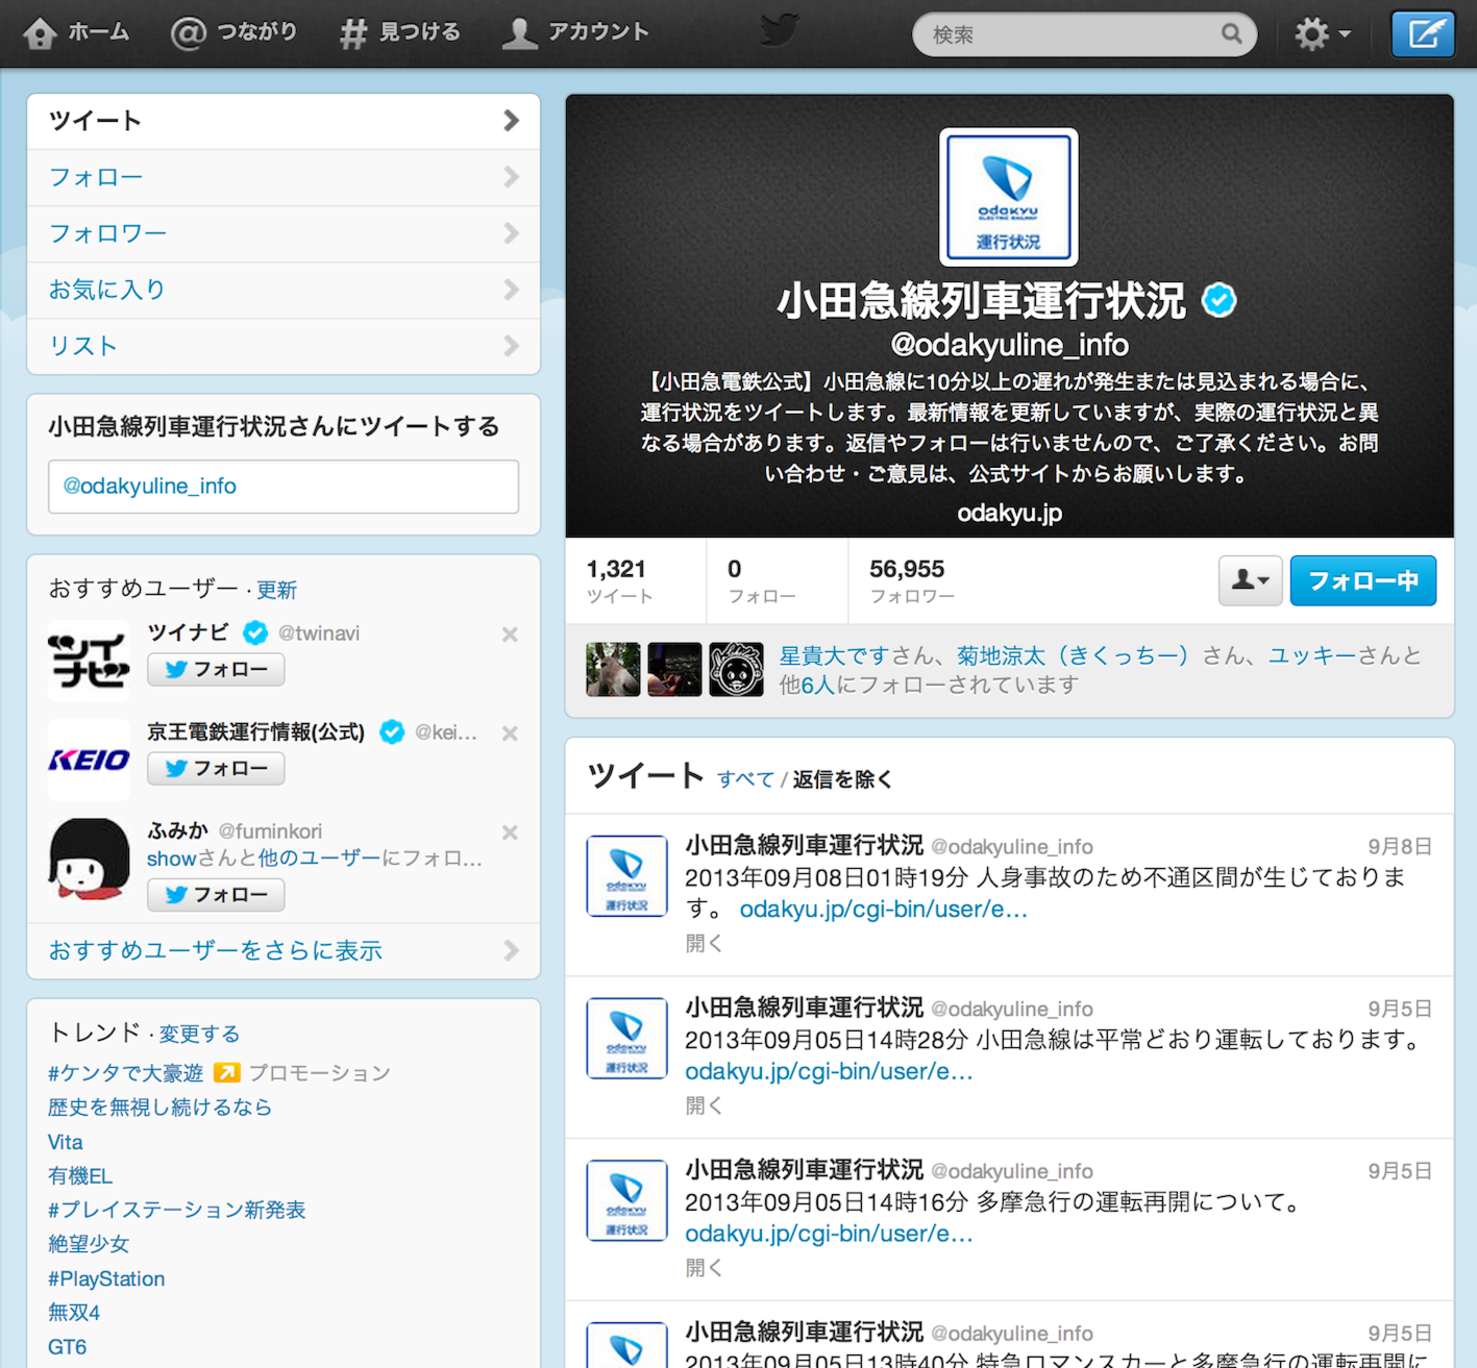
\includegraphics[scale=0.60]{./pdf/odakyu_twitter_page}
      \vspace{-5mm}
      \caption{���ĵ���Twitter��������ȥڡ���}
      \label{fig:odakyu_twitter_page}
    \end{center}
\end{figure}

�ż֤��ٱ�䱿�Ը���碌�ʤɤˤ�äơ�����ɽ�̤�α��Ԥ�Ԥ��Ƥ��ʤ�����
��¿�����롥�ٱ�䱿�Ը���碌���Ф��ơ���Ŵƻ��Ҥ��͡����б���ԤäƤ�
�롥�ꥢ����б��Ȥ��Ƥϡ��Ź��Ǽ��Ĥ˾�����ɽ����ؤ��ٱ����������ۤ�
�ɤ��Ԥ��Ƥ��롥�ꥢ����б��Ϥ��ξ�˹Ԥ��ʤ�����ż֤α��Ծ������Τ�
���Ȥ��Ǥ��ʤ����ᡤ���ѼԤˤȤäƤϤȤƤ��Թ礬���������Τ��ᡤ�ؤ˹Ԥ�
�����ż֤α��Ծ������ǧ�Ǥ���褦�˳�Ŵƻ��Ҥϥ���饤��Ǿ����ȯ����
�Ƥ��롥����饤��Ǥξ���ȯ���λ�����ʲ��˵󤲤롥
\begin{description}
\item {(1)} ���������Ȥˤ����ֱ��Ծ����󶡥ڡ���\\
����Ŵƻ��ҤϤ��줾��Web�����Ȥ���äƤ��뤳�Ȥ�¿����������Web������
�Ǥϴ�Ⱦ��󡤥˥塼�����õޥ����åȤ�ͽ��ʤ��͡��ξ���ȯ������Ƥ��롥
�����ξ����1�ĤȤ��ơ���֤α��Ծ�����ȯ�����Ƥ���ڡ�����¸�ߤ��롥
��\ref{fig:jr_delays_page}\cite{jr:service_status}�Τ褦�˱ؤ˹Ԥ�������
�֤α��Ծ�����Τ뤳�Ȥ��Ǥ��롥���Υڡ����򤦤ޤ����Ѥ���С����٤��Ƥ�
��ϩ������򤷥���������Ȥ��ʤɱؤ˹Ԥ����˺����η�ϩ�����򤹤뤳�Ȥ���
���롥���������������⤢�롥��������Ȥ������Ȥ⤢���ٱ�䱿�Ը���碌��
�ɤ�ȯ�����Ƥ����ۿ��ޤǻ��֤�������Ȥ������Ǥ��롥���Τ��ᡤ����ο���
���Ϲ⤤���ꥢ�륿�����˳������
\item {(2)} Twitter�������������\\
��Twitter�˸�����������Ȥ���äƤ���Ŵƻ��Ҥ⤢�롥���Υ�������Ȥ�ե�
�������뤳�Ȥˤ�äơ�Twitter���äƤ���桼����Twitter�򸫤Ƥ�������ż�
�α��Ծ�������뤳�Ȥ��Ǥ��롥\ref{fig:odakyu_twitter_page}\cite{twitter:odakyu}
���������������⤢�롥������������ȤʤΤǾ��������Τ�ΤʤΤǡ�����
�����ƤޤǤ˻��֤�������ޤ����ޤ�����Ƥ�������ϼºݤ�ȯ�����Ƥ�
���ٱ���⾯�ʤ���
\end{description}


\section{SNS}
SNS�Ȥϡ����������ͥåȥ���󥰥����ӥ���Social Networking Service�ˤ�
ά�Ǥ��롥�Ҳ�Ū�ͥåȥ����Web��˹��ۤ��뤳�ȤǤ��뤬�����ӥ��ڤӥ�����
�Ǥ��롥����Ū�ʵ�ǽ�Ȥ��ơ��ץ��ե����뵡ǽ����å�������ǽ���桼���֤ˤ�
������ߥ�󥯵�ǽ�ȸ�����ǽ���֥�����ǽ�����ߥ�˥ƥ���ǽ�ʤɤ����롥���
����ü������ڤˤ�äơ���ڤ����Ѥ��뤳�Ȥ���ǽ�ˤʤ�¿���οͤ˳��Ѥ����
���롥�����Ǥ�Facebook��Twitter��Google+�����ܤǤ�Mobage��GREE��Ameba��mixi
�ʤɤ����ꡤ¿���οͤ����Ѥ���Ƥ��롥

\subsection{��������륻�󥵤Ȥ��Ƥ�SNS}
�������SNS�桼����������SNS���̤����͡��ξ����ȯ�����Ƥ��롥��ʬ�伫ʬ��
����ξ������̿����ɤ���˥塼���ε����ʤɤ���Ƥ��뤳�Ȥˤ�äơ�SNS���
¾�Υ桼���˸����ƾ����Ȼ����Ƥ��롥�ޤ�SNS�ξ���ȯ�����Ȼ����ԡ��ɤϥƥ�
�ӡ��饸������ʹ��������Ҥʤɤ���ٰ���Ū���ᤤ��This just in��News no 
longer breaks, in Tweets�Ϥ���IT���󥵥륿��Ȥ������ޡ��ӥ󡦥�ǥ���
�������줿�ݡ����ΰ����Ͻ���Twitter�˥ꥢ�륿�������Ƥ��Ƥ������Ȥ򵭻�
�ˤ�����ΤǤ��롥����Ǥ���С����Ԥ��ܿͤ˼�ष�����ˤ��ƴ�¸�Υ�ǥ���
���̤��ƥ˥塼���Ȥ����������˸��������Ϥ��Ǥ��ä�����������Twitter����
���ƥꥢ�륿����˾���ȯ�����Ȼ����줿���Ȥˤ�äơ��Х饯�����Х���������
�۵�������ȯɽ�������ޡ��ӥ󡦥�ǥ���򻦳��������Ȥ����餫�ˤ�������¿��
�οͤ����Τ��Ȥ��ΤäƤ��������λ��¤�Twitter�ʤɤ�SNS���ꥢ�륿��������
�⤤����ȯ�����ΤǤ��뤳�Ȥ������������Ǥ��롥��������̺ҤǤ�Twitter��
facebook���οͤ��²�ΰ��ݡ��Ͽ̤��ﳲ�������ż֤α��Ծ����ˤĤ��Ƥξ���
�����μ��ʤȤ��ƤȤƤ���פ�����̤���������ǯ�Ǥϡ��ͤ�ʪ�����󥵤�Ʊ��
�ε�ǽ����İ��Υ��󥵤ȹͤ�������������ǥ�������Ѥ��ƥꥢ�륿�����
���������¬����Ȥ����ͤ������ޤ줭�Ƥ��롥

%http://jp.techcrunch.com/2011/05/02/20110501news-of-osama-bin-ladens-death-spreads-like-wildfire-on-twitter/


\section{�ӥå��ǡ���}
�ӥå��ǡ����Ȥϡ�����Υǡ����١��������ġ����ǡ����������ץꥱ����
���ǤϽ�������Τ�����ʤۤ����̤ʥǡ�������Τ��ȤǤ��롥

\subsection{�ӥå��ǡ�������ħ}
�ӥå��ǡ�������ħ�Ȥ���3V�Ȥ������դ����롥3V�Ȥϡ��ӥå��ǡ���������
��Value�ˡ������Variety�ˡ����١�Velocity�ˤ�3�Ĥ���ħ�Τ��ȤǤ��롥
�ʲ��Ǥ��줾�����ħ�ˤĤ����������롥
\begin{itemize}
\item ���̡�Volume��\\
��ǯ����Х���ü������ڤ�ȼ��¿���οͤ����󥿡��ͥåȤ���Ѥ���褦��
�ʤä������Τ��ᡤ���󥿡��ͥåȤ����Ѥ����ǡ���������ˤʤäƤ��Ƥ�
�롥����������SNS�Ǥ���facebook��2012ǯ8�������500TB�Υǡ���������
���Ƥ��롥Twitter��2011ǯ10�������1����2��5000���ĥ����Ȥ����ˤ��Ƥ�
�롥140ʸ���θġ��Υĥ����ȤΥǡ����̤���200�Х��ȤʤΤǡ�Twitter��1��
����8�ƥ�Х��Ȥ�Υǡ��������߽Ф��Ƥ���Ȥ������Ȥˤʤ롥�ޤ���Google
��2008ǯ������1����20�ڥ��Х��Ȥ�Υǡ�����������Ƥ��롥��ǯ������٤ơ�
�����ǡ���������ˤʤäƤ��Ƥ���Ȥ��������ӥå��ǡ�����Volume�Ȥ�����ħ
�Ǥ��롥
\item �����Variety��\\
��ǯ������٤ơ����󥿡��ͥåȤ��͡��ʼ���Υǡ��������Ѥ����褦��
�ʤäƤ��Ƥ��롥�ǡ����μ����Web�Υ����ǡ������ƥ����ȥǡ�����������
ư�衤�������ä䥿�֥�å�ü����GPS��Global Positioning System�ˤʤ�
�������˴�����Ƥ����褦�ʥǡ��������Ѥ����褦�ˤʤäƤ��Ƥ��롥��
�˶�ǯ�������Ƥ��Ƥ���Τ������󥿡��ͥåȾ�Υƥ����ȥǡ��������־�
�󡤥����������������󥵥ǡ�����ư��ʤɽ���μ�ή�Ǥ��ä���졼����
�ʥ롦�ǡ����١����Ǥϰ������Ȥ��������¤�ǡ����Ǥ��롥���������
��¤�ǡ�����¸�ߤ������Ѥ���Ƥ��������������ߤϤ���ñ�����Ѥ����
���ǤϤʤ���ʬ�Ϥ��뤳�Ȥˤ�ä�ͭ�Ѥ��θ������褦�Ȥ��������ӥå���
������Variety�Ȥ�����ħ�Ǥ��롥
\item ���١�Velocity��\\
���󥿡��ͥåȾ�����Ѥ����ǡ�����ȯ�����٤��������١�����Ū����
���Ƥ��롥����Υ���ӥ˥��󥹥��ȥ���ȯ������POS��Point Of Sales��
�ǡ�����EC�����Ȥǥ桼���������������뤿�Ӥ�ȯ������Web�Υ���å�����
�꡼��ǡ�����Twitter����Ƥ����ƥ����ȥǡ������ƻ륫����ư�衤��
���ƻϩ�����֤���Ƥ���ƻϩ�ν��ڸ��Υ��󥵤���������¬�ꤹ�륻��
�ʤɤΥ��󥵥ǡ�����Suica��PASMO�ʤɤθ��̷Ϥ�IC�����ɤ������߽Ф���
��������ǡ������Żҥޥ͡��η������ǡ����Ǥ��롥���Τ褦��365��24
�������̤Υǡ��������߽Ф�³���Ƥ���Ȥ��������ӥå��ǡ�����Velocity
�Ȥ�����ħ�Ǥ��롥
\end{itemize}

\subsection{�ӥå��ǡ�����٤��뵻��}
\label{background:bigdata:technology}
�ӥå��ǡ���������ˤʤä��Τ�ñ�˥ǡ������̡����ࡤ���٤������������Ǥ�
�ʤ����ӥå��ǡ����������ʤΥ����Ф��Ѥ������Ѥ�����®�˽������뤳�Ȥ���
���륪���ץ󥽡����Υ��եȥ��������Ѥ����߽Ф��줿���Ȥ��礭���װ���1�Ĥ�
���롥�ʲ��ǥӥå��ǡ���������Ȥʤä��װ��ε��Ѥ������򤹤롥
\begin{itemize}
\item Hadoop\\
Hadoop�Ȥϡ�Apache����ȯ�������ץ󥽡����Ȥ��Ƹ������Ƥ����絬��ʬ������
�ե졼�����Ǥ��롥Hadoop�ϥ��ץꥱ������󤬿���Ρ��ɤ���ӥڥ��Х�
�ȵ�Υǡ�����������뤳�Ȥ���ǽ�Ǥ��롥Hadoop��Google����ȯ����MapReduce��
Google File System��GFS�ˡ�Big Table���Ȥ˳�ȯ���줿��Hadoop��MapReduce��
Hadoop Distributed File System��HDFS�ˡ�HBase���鹽������롥MapReduce�Ȥϡ�
����ʥǡ������åȤ��Ф������������ǽ�������Map���ƥåס�Reduce���ƥå�
�ǽ����򤹤���������Τ��ȤǤ��롥MapReduce��ʣ����Υ����Ф˽�����ʬ����
���뤳�Ȥˤ�äơ�1��Ǥϲ����⤫���äƤ�������������֤ǽ������뤳�Ȥ���
ǽ�ˤʤä���
\item NoSQL\\
NoSQL�Ȥϡ�Not only SQL��ά�Ǥ��롥���褫��ǡ��������Ȥ��ơ���졼����ʥ�
�ǡ����١������������ƥ��RDBMS�ˤ����Ѥ���Ƥ��롥RDBMS�ϡ�SQL�Ȥ���ɸ���
��ˤ�äƥǡ����١���������Τ��Ф��ơ�NoSQL��SQL����Ѥ��ʤ���NoSQL��
RDBMS�����ꤷ�ƤǤ�����ΤǤϤʤ���RDBMS�����դǤϤʤ����Ȥ�¹Բ�ǽ�ˤ���
�ǡ����١����Ǥ��롥RDBMS��NoSQL�ΰ㤤��ʲ��˵󤲤롥
    \begin{itemize}
    \item[��1��] �ǡ�����¤\\
    RDBMS�Ǥϡ��ǡ�����ơ��֥�Ȥ���ɽ�����ǽ��󤷡��ǡ���Ʊ�Τδط�������
    �����롥�������뤳�ȤǸ��ʤʥǡ�����ǥ��ɽ�����Ƥ��롥���Τ���ơ��֥�
    �Υ����������������Ƥ���ɬ�פ����롥������������������ޤϸ���Ū�Ǥ�
    ���ѹ����ˤ�����
    NoSQL�Ǥϡ��������б�����Х�塼���Ȥ߹�碌�����뤤�ϡ��������Х�塼
    �Υڥ����ɲå����ʥ����ե��ߥ꡼�ˤˤ�ä�ɽ������뤿�ᡥ�ǡ�����¤��
    �ȤƤ�ñ��Ǥ��롥�ǡ���Ʊ�Τδط���������뤳�Ȥ��Ǥ��ʤ����������ޤ���
    ������ɬ�פ��ʤ�������ѹ���ǽ�Ǥ��롥
    \item[��2��] �ǡ����ΰ����\\
    RDBMS�Ǥϡ�ACID��Atomicity Consistency Isolation Durability������������
    ����Ƥ��뤿�ᡤ�ǡ����ΰ��������̩�˰ݻ�����Ƥ��롥������NoSQL�ǡ���
    �١����Ǥ�ACID�Τ褦�ʷ�ϴ�ʤ�ΤǤϤʤ���Eventual Consistency�Ȥ�������
    �ˤʤäƤ��ꡤ�ǽ�Ū�˰�������ݻ�����뤬�����Ū�ˤϰ��������̩�Ǥ�
    �ʤ���
    \item[��3��] ��ĥ��\\
    RDBMS�ξ�硤ACID��ǡ�����¤��Ż뤹�뤿�ᡤ�ǡ����̤��������Ȥ��Ϥ��
    �礭�ʥ����Ф��Ѥ��륹�����륢�åפ����ܤǤ��ꡤ�������륢���Ȥ��ˤ���
    �������ƥ�����ȤʤäƤ��롥�ޤ����ǡ����ΰ������̩�˹Ԥ�����ѥե���
    �ޥ󥹤��㲼�ⵯ�롥NoSQL�ǡ����١����ξ�硤�������륢���Ȥ��ưפˤǤ���
    �߷פˤʤäƤ��뤿���ĥ����ͥ��Ƥ��롥�ޤ����ѥե����ޥ󥹤��㲼�⾯�ʤ���
    \item[��4��] �Ѿ㳲��\\
    RDBMS�ϥ�ץꥱ�������ˤ�äơ�ʣ���Υ����Ф˥ǡ�����ʣ�����Ѿ㳲����
    ���Ƥ��롥���������ǡ����������礬���ä������ץꥱ���������ɲ�
    ����ݤˤϱ��Ѿ����٤䥳���Ȥ��礭����NoSQL�ξ�硤ʬ���Ķ���ư���
    ���ᡤñ��㳲�����ʤ���Τ�¿�����㳲���Ф����к������Ȥ����ʤ��Ѥࡥ
    \end{itemize}
�ʾ�Τ褦�ˡ�NoSQL��RDBMS�����դǤϤʤ����Ȳ�褹����ħ��¿����
\item ���饦�ɥ���ԥ塼�ƥ���\\
���饦�ɥ���ԥ塼�ƥ��󥰤Ȥϡ��ͥåȥ���������С����ȥ졼�������ץꥱ��
����󡤥����ӥ��ʤɤι�����ǽ�ʥ���ԥ塼�ƥ��󥰥꥽�����ζ�ͭ�ס�����Ф��ơ�
�������ĥ���ǥޥ�ɤ˥��������Ǥ����Ǿ��δ���ϫ�Ϥޤ��ϥ����ӥ��ץ��Х����֤�
���ư��ˤ�äƿ�®���󶡤������ѤǤ���Ȥ�����ǥ�ΤҤȤĤǤ���ȡ�����ꥫ
��Ωɸ�ൻ�Ѹ�����������Ƥ��롥����Ǥ���С���ʬ���Ȥ�ʪ��Ū�ʥ����Ф��Ѱ�
�����ǡ�����������ʤ��ƤϤʤ�ʤ��ä��������ǡ����̤�¿���ʤ�Фʤ�ۤ�ɬ�פ�
�꥽������¿�����ꡤ���Ƥ��������ΤϤȤƤ����ѤǤ��롥���������饦�ɥ���ԥ�
���ƥ��󥰤ε��Ѥ�ȯã�������Ȥˤ�äơ����ѼԤ�ʪ��Ū�ʥ꥽������ǡ���������
�Ĥ��ƹͤ���ɬ�פ��ʤ��ʤꡤ���������Ǥ��륵���ӥ��並��˽��椹�뤳�Ȥ���ǽ
�ˤʤä����ޤ������̤����Ѥ���������ʧ���Ȥ��������Ǥ��ꡤ���ܤξ��ʤ���������
���å״�Ȥ�ĿͤǤ��ڤ����Ѥ��뤳�Ȥ��Ǥ��롥�����ߵ���㤵�����ӥå��ǡ���
���Ѥ��礭���׸����Ƥ����װ��Ǥ��롥
\end{itemize}

\section{�ӥå��ǡ����γ���}
�ӥå��ǡ������͡��ʾ��̤dz��Ѥ���Ƥ��롥���ʤ䥵���ӥ��Υ쥳���ǡ������
��ư�������ƥ��󥰹��𡤰۾︡�Ρ������ӥ��β��������ڤ�ͽ¬�����٤�ͽ¬������
��ͽ¬�ʤɳ��Ѥ�����оݤ����������ӥå��ǡ����γ��ѥѥ�������礭��ʬ����2��2��
4�ĤΥѥ�������෿���Ǥ��롥���ϡָĿͺ�Ŭ/���κ�Ŭ�ס֥ꥢ�륿���෿/�Хå�����
�Ǥ��롥�Ŀͺ�Ŭ�Ȥϡ�ʬ�Ϸ�̤μ��׼Ԥ�����θĿͤ��ΤǤ��ꡤ����θĿͤ���
�ˤȤäƺ�Ŭ�ʾ���䥵���ӥ����󶡤����ꡤ��Ŭ�ʽ�����¥����ΤǤ��롥���κ�Ŭ
�Ȥϡ�ʬ�Ϸ�̤μ��׼Ԥ�����θĿͤ��ΤǤϤʤ������θĿͤ��Τ�°���륳�ߥ�
�˥ƥ������뤤�ϼҲ����Τʤɥޥ��ξ��Ǥ��롥���줾��ˤĤ��ưʲ����������롥

\subsection{�ӥå��ǡ����γ��ѥѥ�����}
�����Ǥ����Ĥ���ʸ�䥵���ӥ������󤲤�ͽ�ꡪ\\
\\
\begin{itemize}
\item �Ŀͺ�Ŭ���Хå���\\
�Ŀͺ�Ŭ���Хå����Ȥϡ�����θĿͤ��Τ˴ؤ���ǡ�����������ơ����οͤ˺�Ŭ
�ʾ��ʤ䥵���ӥ���쥳���ɤ����ꡤ���Υ�Τ˺�Ŭ�ʽ��֤�Ԥä��ꤹ����Ǥ�
�롥��ɽŪ�ʥ����ӥ���Amazon�Ǥ��롥Amazon��¿���Υ桼���ι������򡤱��������
���������Ϲ��λ��Ƥ���桼���򥰥롼�ײ������Ϲ��λ��Ƥ���桼���ξ��󤫤龦��
��쥳���ɤ��Ƥ��롥�������뤳�Ȥ����ѼԤ˲��ͤΤ��������󶡤���������¥��
���Ƥ��롥����϶�Ĵ�ե��륿��󥰤Ȥ����쥳���ǡ�����󥢥르�ꥺ��Ǥ��롥
\item �Ŀͺ�Ŭ���ꥢ�륿���෿\\
�Ŀͺ�Ŭ���ꥢ�륿���෿�Ȥϡ�����θĿͤޤ��ϥ�Τ˴ؤ���ǡ����������������
�ͤ˺�Ŭ�ʾ��ʤ䥵���ӥ���쥳���ɤ����ꡤ���Υ�Τ˺�Ŭ�ʽ��֤�Ԥä��ꤹ��
���Ǥ��롥���������Хå����Ȥϰۤʤꡤ���οͤ˾��ʤ䥵���ӥ���쥳���ɤ���
�ꡤ���Υ�Τ˺�Ŭ�ʽ��֤�ܤ������ߥ󥰤ϥ���ƥ����Ȥ˹�碌�ƥꥢ�륿�����
�Ԥ��롥
\item ���κ�Ŭ���Хå���\\
���κ�Ŭ���Хå����Ȥϡ�¿���θĿͤ��Τ�ȯ������������������Ѥ������Ѥ���
�ǡ������礷������Ū�˽�����ʬ�Ϥ��뤳�Ȥǡ����θĿͤ��Τ�°���륳�ߥ�˥�
����Ҳ����ΤˤȤä���Ω�����׾����ե����ɥХå������ꡤ��Ŭ����ޤ�����
��������������Ŭ�������ꤹ�륿���ߥ󥰤����ʤ���
\item ���κ�Ŭ���ꥢ�륿���෿\\
���κ�Ŭ���ꥢ�륿���෿�Ȥϡ�¿���θĿͤ��Τ�ȯ������������������Ѥ�����
�Ѥ����ǡ������礷������Ū�˽�����ʬ�Ϥ��뤳�Ȥǡ����θĿͤ��Τ�°���륳��
��˥ƥ���Ҳ����ΤˤȤä���Ω�ľ���򥳥�ƥ����Ȥ˹�碌�ƥꥢ�륿����˥ե�
���ɥХå������ꡤ��Ŭ��������Ǥ��롥
\end{itemize}

\section{����ʸ�������}
��\ref{background:railroads:problems}�����\ref{background:railroads:correspondence}��
�ǽҤ٤��̤ꡤ�ż֤ˤ��ٱ䡤��ž����碌�������б������꤬���롥������
�ż����ѼԤ��ޤ��ٱ�䱿ž����碌�Ǻ��𤷤ʤ��褦�ˡ��ꥢ�륿�������
�֤Υ�����������Τ���ˡ��ɬ�פǤ��롥�ܸ���Ǥϡ�Twitter�桼����1��
�Υ��󥵤Ȥ��Ƥߤʤ���ȯ��������ż֤˴ؤ���ƥ����ȥǡ�������\ref{background:bigdata:technology}��
�������������Ѥ��Ѥ��Ƽ��������ѡ�ʬ�Ϥ��뤳�Ȥˤ�äơ���֤α��Ծ���
���˥���󥰤����桼�����󶡤��륢�ץꥱ��������ȯ���롥Twitter
����Ѥ�����ͳ�ϡ��ꥢ�륿��������Ż뤹�뤿��Ǥ��롥

\section{�ޤȤ�}
�ܾϤǤϡ��ż֤��ٱ䡤���Ը���碌�������б������꤬���뤳�Ȥ򼨤�����
�ޤ��ӥå��ǡ����γ�ǰ�ˤĤ��ƽҤ١��ӥå��ǡ�������Ѥ��뤳�Ȥˤ��
�ơ�������͡���������褷������䥵���ӥ���󤲤����ܸ���Ǥϡ�
Twitter����Ƥ��줿�ż֤˴ؤ���ĥ����Ȥ���������ѡ�ʬ�Ϥ��뤳�Ȥ�
��äơ���֤α��Ծ������˥���󥰤����桼�������Τ��륢�ץꥱ��
�����γ�ȯ���ܻؤ���

%%% Local Variables:
%%% mode: japanese-latex
%%% TeX-master: "../nakajima_bthesis"
%%% End:

\chapter{��Ϣ����}
\label{related_works}

%%% Local Variables:
%%% mode: japanese-latex
%%% TeX-master: "../nakajima_bthesis"
%%% End:

\chapter{��Ƽ�ˡ}

\section{�ͥåȥ�������Ԥȼ�������}

\subsection{����}

\subsection{�ѥ��åȤΥإå�����}

\subsection{�ۥ��ȼ��̤ˤ��Ĵ��}



\section{Ʊ�쥻�����Ⱦ�Υ桼���ȼ�������}

\subsection{����}

\subsection{��ͭ�ۥ���̾}



\section{�軰�ԤǤ���桼���ȼ�������}

\subsection{����}

\subsection{Bluetooth}



\section{�ޤȤ�}


%%% Local Variables:
%%% mode: japanese-latex
%%% TeX-master: "../nakajima_bthesis"
%%% End:

\chapter{����}
\section{section1}

\section{section2}

\section{section3}


\chapter{ɾ��}

\section{ɾ����ˡ}

\section{���ƥ١���ʬ�����ʬ��ɾ��}

\section{������ʬ����ʬ��ɾ��}

\section{�ٱ�ȯ���������ΤޤǤλ��֤�ɾ��}

\section{�ޤȤ�}

%%% Local Variables:
%%% mode: japanese-latex
%%% TeX-master: "../nakajima_bthesis"
%%% End:

\chapter{����}
\label{conclusion}

\section{�ޤȤ�}
\label{conclusion:matome}

\section{�����Ÿ˾}
\label{conclusion:matome}

%%% Local Variables:
%%% mode: japanese-latex
%%% TeX-master: "../nakajima_bthesis"
%%% End:

\chapter*{�ռ�}
\addcontentsline{toc}{chapter}{�ռ�}
\label{thanks}
����ʸ�κ����ˤ����ꡤ����Ƴĺ�������������شĶ������������
Ĺ ¼�� ����Ρ�Ʊ�������� ���� �ѹ���Ρ�Ʊ�������� ��¼ ����Ρ�Ʊ����
�ڶ��� ���� ��Ƿ��Ρ�Ʊ�����ڶ��� �⼮ �쵪��Ρ�Ʊ�����ڶ��� ���� ��
��Ρ�Ʊ�����ڶ��� ���� ������Ρ�Ʊ������Ǥ�ֻ� �Ŷ� �Ϲ���Ρ�Ʊ����
��Ǥ�ֻ� ��߷ ����Ρ�Ʊ������Ǥ�ֻ� Rodney D.Van Meter III ��Ρ�Ʊ��
������ ���� ������Ρ�Ʊ���DMC������Ǥ�ֻ� ��ƣ ������Ρ�Ʊ���������
��ǥ�����������̸���ֻ� ��ƣ ������Τ˴����פ��ޤ����ä����ķ�����
�Τϡ�����ǹԤ��ͤޤ����Ф������˺���������Ƴ���Ƥ��������ޤ�����
��˿����������ǥ����ȸ����ˡ�ǻ��Ƴ���Ƥ������������٤��˿�������
������ܤ򸫤��Ƥ��������ޤ����������ˤ��꤬�Ȥ��������ޤ�����

�����ơ��ܸ����ʤ�Ƥ�����ǡ��͡�����ޤ��Ƚ��������������򤤤�������
������¼�渦�漼´�����Ǥ�����¼ ͧ��ᡤ��� �ͻᡤ��¼ ʹ��ᡤ���� �ɻᡤ
�и� ���λᡤ��Τ �ûᡤ���� δμ�ᡤ���� �ҹ���˴����פ��ޤ���

������������ر���ǥ����ǥ����󸦵����β������� δ�˻ᡤƱ���������
��ǥ�������ʸ����β��� ���� �̻ʻᡤ�پ� �����ᡤ�ĺ� �ϻᡤ��ƣ ��
�ƻᡤ�׾� ��ᡤ���� �µ׻ᡤ���� �¹��ᡤ��ë ���Ļᡤ��ë ��˻ᡤ��
�� ��ʿ�ᡤƱ����ʽ��β�����ϻ�� ��ʹ�ᡤ���� ���ᡤ��¼ ����ᡤ��
�� ͤ��ᡤ��ƣ ζ��˴����פ��ޤ����ä˿�ë ���Ļ�ϡ������ʸ�μ�ɮ��
�ز�ȯɽ��¿˻�ʿȤˤ�ؤ�餺���ƿȤ����̤˾�äƤ����������������������
��Ƴ������κ٤䤫�ʥ�����Ϥ���Ȥ��뤢�����̤����ݤ򸫤Ƥ���������
��������ʤ��Ǥ�´����ɮ�����Ǥʤ����¤������漼���������ޤ���Ǥ�����
�����˴����פ��ޤ���

����˶��Ϥ򤷤Ƥ��������������� ����ᡤ��¼ �˻ᡤʡ�� ��ů�ᡤ��
�� ������ᡤ���� ���ᡤDoan Viet Tung�ᡤ���� ����ᡤ���� ���ƻᡤ
�긫 ���˻ᡤ��� ���ᡤƣ�� ζ�ᡤ�ȸ� ��ƻ�ᡤ��߷ �ߤ椭�ᡤߧ�� ��
��ᡤ¼�� ����������ġ�¼���Ʊ���漼�γ��͡�������´����ɮ�����Ǥ�
����DSAP09���С��˴����פ��ޤ���

���漼�Ƕ�ڤ򶦤ˤ����ʻ� �����ᡤ��ƣ ��ɧ�ᡤ��¿�� �����ᡤ���� ͧ��ᡤ
ī�� ���һ�˴����פ��ޤ������Ȱ��˸���򤹤뤳�ȤǤ��ߤ���ɷ㤷��
���������ι⤤�����並��򤹤뤳�Ȥ��Ǥ��ޤ�����

������4ǯ�֤ο��ε���Ǥ��ä�SFC���ڥ��������������� ��Τ�һ��Ϥ�
��Ȥ������������˿����鴶���פ��ޤ���´����ɮ�򤹤����Ȥ��������³
���Ƥ��줿�ǥ󥹥��ȡ���˾���¤ޤ��Ƥ��줿��Ĺ�˴��դ��ޤ������Τ�
�����ǿ���;͵���ä�´����ɮ�Ǥ����ȳο����Ƥ��ޤ���

�Ǹ�ˡ�������ؤ����4ǯ�֤����Ǥʤ�22ǯ�֤򤢤����̤ǻ٤��Ƥ����������㡤�帶 �򻰡�
�졤�帶 ���ҤȻ�β�²�˿����鴶���פ��ޤ���


%%% Local Variables:
%%% mode: japanese-latex
%%% TeX-master: "../nakajima_bthesis"
%%% End:


\renewcommand{\thechapter}{\Alph{chapter}}
\setcounter{chapter}{0}
\vspace{-5mm}


\bibliographystyle{unsrt}
\bibliography{./bib/track,./bib/privacy,./bib/company,./bib/software,./bib/railroad}
\thispagestyle{empty}%bibtex


\end{document}

